\documentclass[17pt]{flash}
\usepackage{tkz-euclide}
\startdatakeys
\cycle{}
\connaissancesRequises{}
\competencesTravaillees{}
\enddatakeys
\begin{document}

\flashvisibletimertrue
\FlashSetItemSep{0pt}
\FlashSetVtop{-5em}
\FlashSetTitle{Calcul posé}

\FlashShowConsignes{%
        \item Pour chaque question écrire la grandeur associée à la valeur.
}
\def\docfontsize{\small}
\flash{180}{\docfontsize
    \def\lenght{7}
    \def\height{3}
    \def\unit{m}
    \begin{minipage}{.65\linewidth}
        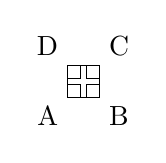
\begin{tikzpicture}[scale=0.4]
            \coordinate[label=below left:A](A)at(0,0);
            \coordinate[label=below right:B](B)at(\lenght,0);
            \coordinate[label=above right:C](C)at(\lenght,\height);
            \coordinate[label=above left:D](D)at(0,\height);
            \draw(A)--(B)--(C)--(D)--cycle;
            \tkzMarkRightAngle[size=0.4](A,B,C)
            \tkzMarkRightAngle[size=0.4](B,C,D)
            \tkzMarkRightAngle[size=0.4](C,D,A)
            \tkzMarkRightAngle[size=0.4](D,A,B)
            \path(A)--(B)node[midway,below,sloped]{\lenght\ \unit};
            \path(B)--(C)node[midway,right]{\height\ \unit};
        \end{tikzpicture}
    \end{minipage}%
    \begin{minipage}{.35\linewidth}
        \begin{enumerate}[label=\alph*),font=\bfseries]
            \item \lenght\ \unit
            \item \height\ \unit 
            \item \number\numexpr2*(\lenght+\height)\ \unit
            \item \number\numexpr\lenght*\height\ \unit$^2$
            \item 90$^\circ$
        \end{enumerate}
    \end{minipage}
}
\def\docfontsize{\footnotesize}
\FlashCorrection

\end{document}